\documentclass[a4paper,12pt]{article}
\usepackage[utf8]{inputenc}
\usepackage[english]{babel}
\usepackage{blindtext}
\usepackage{authblk}
\usepackage{graphics}
\usepackage{graphicx}
\usepackage{mathptmx}
\usepackage[singlespacing]{setspace}
\usepackage[margin=1in]{geometry}
\graphicspath{{images/}}


\title{IC$^{2}$S$^{2}$ 2018 Submission: Uber's Impact on Flu Infections: An Exploratory Analysis  \\
	\normalsize $4$$^{th}$ International Conference on Computational Social Science IC$^{2}$S$^{2}$ \\
	\normalsize July 12-15, 2018 \\
	\normalsize Northwestern University’s Kellogg School of Management \\
	\normalsize Evanston, IL. USA
}



\author[1]{Anonymous} % Please leave Author-field blank for blind review and remove information that may identify the author(s)
 
\date{}

\begin{document}

\maketitle

\vspace{-2em}

\begin{center}
\textbf{\textit{keywords: Ride-hailing services, behavior and social aspects of health, Google Flu Trends, flu-like illness, natural experiment.  }}
\newline
\end{center}


\section{Extended Abstract}
Ride-hailing services, such as Uber and Lyft, are disrupting the transportation system worldwide having a pronounced impact on people's usage patterns. In 2016, Subway ridership in New York declined for the first time in years, whereas ride-hailing services became the leading source of growth in non-auto travel \cite{schaller2017unsustainable}. However, there are mixed results about the relationship between ride-hailing services and public transportation. For example, a Pew study suggests that ride-hailing is complementary to public transit and walking %\cite{smith2016shared}, while current evidence suggests that ride-hailing is pulling more people away from public transit in cities \cite{clewlow2017disruptive}. One thing is clear: ride-hailing is changing the way we move in cities. 

In this paper, we study the effects of ride-hailing on health related issues, particularly, the spread of flu-related illness. There is evidence suggesting that public transportation is important in the propagation of influenza-like illness in winter \cite{troko2011public,cooley2011role}. Based on these results, we hypothesize that a change in how people commute, as a consequence of ride-hailing services, can have an effect on the contagious levels of influenza in the population. Here, we present one of the first quantitative explorations of the relationship between ride-hailing services and health. We exploit the fact that Uber, the first and most popular ride-hailing platform, was rolled out across the US piecewise and not all at once. Thus, we are provided with an excellent natural experiment setting to identify its impact. Figure \ref{fig:Uber} shows for a sample of cities the dates that UberX and UberPool where introduced.

Unfortunately, weekly US Influenza Surveillance reports are aggregated at a state level and to our knowledge there is no other source that provides finer granularity levels. However, we can rely on Google Flu Trends as a proxy to measure flu-related illness at a city level. Google Flu Trends utilizes internet search queries to detect the presence of influenza like illness and has been use effectively for Influenza forecasting \cite{yang2015accurate}.
%,dugas2013influenza}.

Similar to Berger et al's. paper \cite{berger2017drivers}, where Uber's impact on unemployment was studied, we use a difference-in-differences approach to compare changes in the influenza levels in U.S. cities before and after UberX and UberPool introduction. Our baseline regression model is
\[
y_{it}=city_{i}+year_{t}+month_{t}+\alpha Uber_{it}+\beta Pool_{it}+\gamma X_{it}+ \varepsilon_{it},
\]
where $y_{it}$ is log of the flu estimate for city $i$ and month $t$; fixed effects variables $city_{i}$, $year_{t}$ and $month_{t}$ account, respectively, for time-invariant differences in city baseline levels, city-invariant US yearly pandemic levels, and the seasonality nature of flu. $Uber_{it}$ and $ Pool_{it}$ take the form of a dummy variable representing if UberX and UberPool services are present in city $i$ and month $t$; $X_{it}$ are time varying and city characteristics to control for weather data such as monthly min and max temperatures and monthly precipitation.

We present results for 12 cities: Austin, Boston, Chicago, Houston, Los Angeles, Miami, New York, Philadelphia, Phoenix,  San Francisco, Seattle and Buffalo (Buffalo being one of the few cities without Uber). The weather variables were statistically insignificant as most of their effects are included in the seasonal coefficients, so in the following, we present results of the model without them.
Our model yields the following estimates:  $\alpha =-0.25$ ($p$-value$<10^{-8}$) and $\beta =-0.072$ ($p$-value$=0.075$). Our results suggest that flu-like illness cases have decreased $30\%$ on average after the introduction of Uber relative to other cities. To disentangle further the relative effects of UberX and UberPool, Figure \ref{fig:interaction} shows the monthly interaction terms for each service. Notice  that the effect of UberPool in winter tends to be positively correlated with the number of Flu cases,  while the direction of the effect of UberX is the opposite and almost always negative.

Taken together, we find suggestive evidence that ride-hailing services do have an effect on flu-like illness rates. However, our findings cannot be generalized, as Uber's impact on health is heterogeneous over time and cities. In future research, we plan to extend our regression model to account for autocorrelated errors and use an interrupted time series analysis approach. Furthermore, we will expand the list of US cities included in the analysis and incorporate additional relevant control variables such as public transportation data.




\bibliographystyle{plain}
\bibliography{references}

\newpage
\section{Figures}

\begin{figure}[h!]
\centering
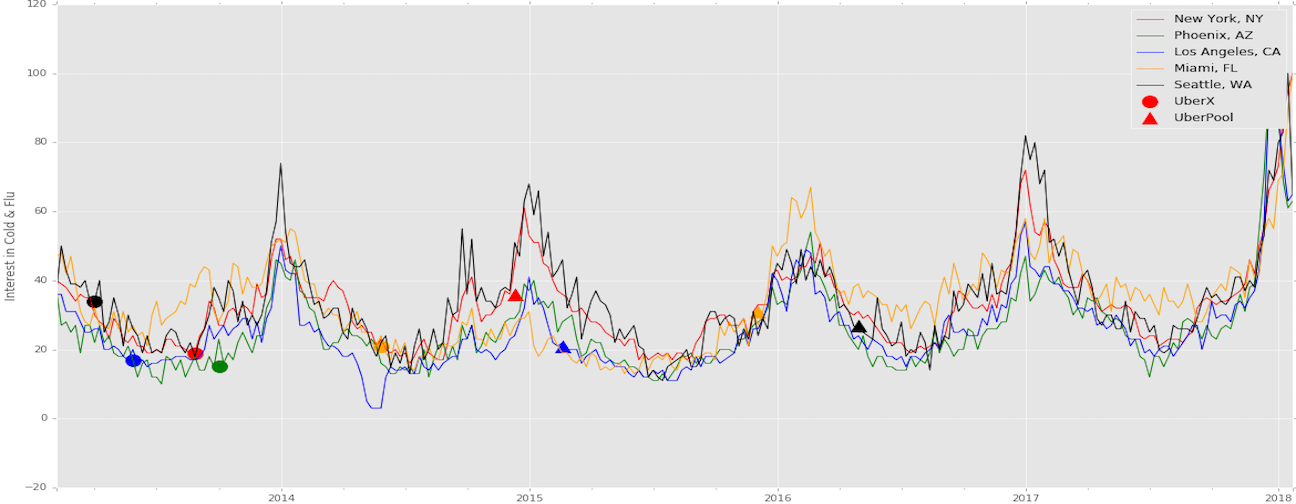
\includegraphics[width=15cm]{images/fig1}
\caption{Google monthly Flu trends over time for various cities. Circle and triangle marks identify the time when UberX and UberPool were introduced for each city, respectively. Uberpool is a share ride service and Uber's most affordable way to travel. }
\label{fig:Uber}
\end{figure}
\begin{figure}[h!]
\centering
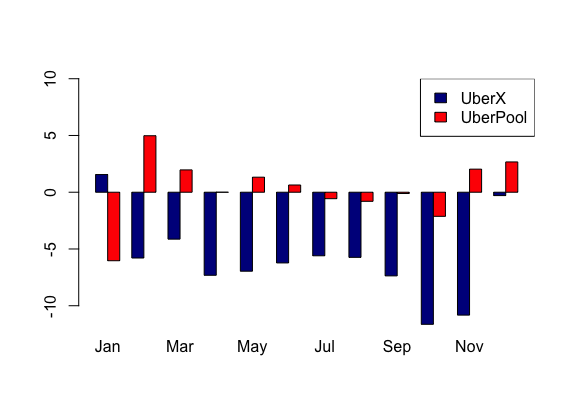
\includegraphics[width=15cm]{images/Coefficients}
\caption{Seasonality dependent impact of UberX and UberPool on Flu cases. Here we depict the monthly interaction terms for variables $Uber_{it}$ and $ Pool_{it}$ in the model.  The values represent the average monthly change in percentages of Flu cases due to the presence of UberX and UberPool. The addition of both terms is the total effect of Uber.     }
\label{fig:interaction}
\end{figure}

\end{document}
